\documentclass[tikz]{standalone}

\usetikzlibrary{calc, positioning, shapes.arrows}

\begin{document}
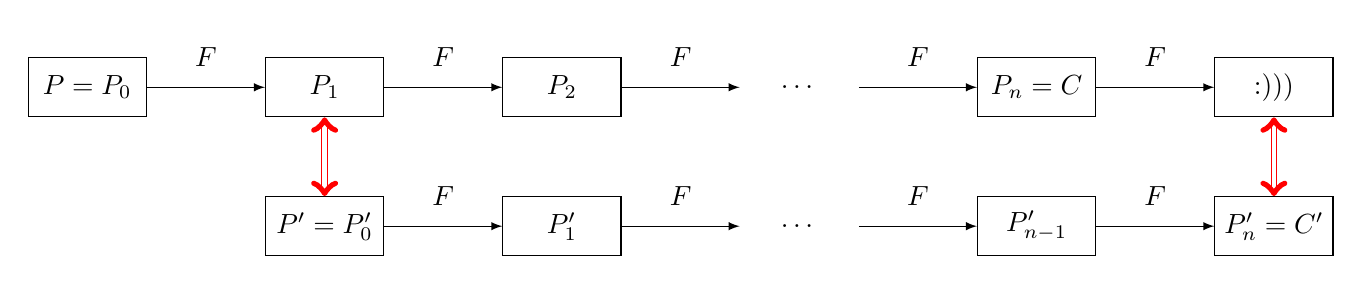
\begin{tikzpicture}[
    every node/.style = {rectangle, minimum width=1.5cm, minimum height=0.75cm}
]
    \node[draw] (P0) {$P = P_0$};
    \node[draw, right=1.5cm of P0] (P1) {$P_1$};
    \node[draw, right=1.5cm of P1] (P2) {$P_2$};
    \node[right=1.5cm of P2] (Pt) {\dots};
    \node[draw, right=1.5cm of Pt] (Pn) {$P_n = C$};
    \node[draw, right=1.5cm of Pn] (Pn+1) {:)))};

    \node[draw, below=1cm of P1] (p0) {$P' = P_0'$};
    \node[draw, right=1.5cm of p0] (p1) {$P_1'$};
    \node[right=1.5cm of p1] (pt) {\dots};
    \node[draw, right=1.5cm of pt] (pn-1) {$P_{n-1}'$};
    \node[draw, right=1.5cm of pn-1] (pn) {$P_n' = C'$};

    \draw[-latex] (P0) -- node[above] {$F$} (P1);
    \draw[-latex] (P1) -- node[above] {$F$} (P2);
    \draw[-latex] (P2) -- node[above] {$F$} (Pt);
    \draw[-latex] (Pt) -- node[above] {$F$} (Pn);
    \draw[-latex] (Pn) -- node[above] {$F$} (Pn+1);

    \draw[-latex] (p0) -- node[above] {$F$} (p1);
    \draw[-latex] (p1) -- node[above] {$F$} (pt);
    \draw[-latex] (pt) -- node[above] {$F$} (pn-1);
    \draw[-latex] (pn-1) -- node[above] {$F$} (pn);

    \draw[<->,double equal sign distance, red] (P1) -- (p0);
    \draw[<->,double equal sign distance, red] (Pn+1) -- (pn);
\end{tikzpicture}
\end{document}